% Provenance (never printed): see sources/outline_sources.md (Year 1: solute and particle
% fluxes; the Hjulstrom diagram; settling velocity; denudation rates). Exercise and problem
% values in the Book 3 scratch calculator calc/ch20.py; figure data from
% figdata/bachelor-1/settling.py and threshold.py. Erosion, transport and deposition are
% Book 1's (g5); the sediment load in three forms, the denudation rate and isostatic rebound
% are Book 2's (g12), re-founded here (load, denudation rate) or recalled (rebound); discharge
% and the drainage basin are Book 2 g10's; Airy isostasy is ch. 11's; viscosity, Stokes' law
% and the Reynolds number are the physics books' (admitted, pointer). Grain-size classes and
% sorting belong to ch. 21.
\chapter{Érosion et transport}\label{ch:b1:erosion-transport}

Après un orage, la rivière sous le pont coule brune. L'eau qui était claire
la veille est épaisse de boue, tourbillonne autour des piles et charrie
des branches, et sur le lit, invisibles, des galets s'entrechoquent en
roulant. Chaque seconde la crue emporte des tonnes de terre. En aval,
derrière un barrage, la même boue se dépose dans l'eau calme du réservoir, qui
perd un peu de son volume chaque année~; plus loin encore, à l'embouchure,
elle s'étale dans la mer en un panache brun visible depuis l'espace. Ce
chapitre met des chiffres sur ce voyage~: combien une rivière transporte et sous quelles
formes, à quelle vitesse un grain coule, quel courant il faut pour le mettre en mouvement, et
à quelle vitesse, au bout du compte, tout un paysage est usé.

\begin{recall}
L'érosion est l'usure de la terre et l'enlèvement des morceaux~;
le dépôt est leur mise à plat là où le porteur ralentit (livre~1, année~5). Une
rivière transporte sa charge sédimentaire sous forme de \omterm{def:b1:erosion-transport:load}{charge de fond}, de \omterm{def:b1:erosion-transport:load}{charge en suspension} et de \omterm{def:b1:erosion-transport:load}{charge
dissoute}~; le \omterm{def:b1:erosion-transport:denudation}{taux de dénudation} d'une région est l'épaisseur de roche enlevée de
celle-ci par unité de temps, en mètres par million d'années~; quand l'érosion enlève une épaisseur
$e$ de \omterm{def:b1:layered-earth:layers}{croûte}, le rebond isostatique ne laisse la surface descendre que de
$e(1 - \rho_c/\rho_m)$ (livre~2, année~12). Le débit d'une rivière est le
volume d'eau qui passe une section par unité de temps, et son bassin versant
l'aire qui l'alimente (livre~2, année~10). Dans l'\omterm{prop:b1:isostasy-gravity:airy}{isostasie d'Airy} la \omterm{def:b1:layered-earth:layers}{croûte}
flotte sur le \omterm{def:b1:layered-earth:layers}{manteau} avec une racine proportionnelle à son relief
(\cref{prop:b1:isostasy-gravity:airy}). L'\omterm{def:b1:weathering-clays:hydrolysis}{hydrolyse} des silicates envoie des ions
et de la silice dissoute aux rivières (\cref{def:b1:weathering-clays:hydrolysis}).
La viscosité dynamique $\mu$ d'un fluide mesure sa résistance au cisaillement,
et la viscosité cinématique est $\nu = \mu/\rho$~; une sphère de diamètre $d$
se déplaçant lentement à la vitesse $w$ dans un fluide subit la traînée $3\pi\mu d w$
(loi de Stokes)~; le nombre de Reynolds $w d/\nu$ compare l'inertie aux forces
visqueuses, et l'écoulement autour de la sphère est lisse tant qu'il reste petit (les
livres de physique).
\end{recall}

\section{Flux de solutés et de particules}\label{sec:b1:erosion-transport:fluxes}

Une rivière enlève la terre de deux façons~: sous forme de matière en solution, les produits de
l'\omterm{def:b1:weathering-clays:weathering}{altération chimique}, et sous forme de grains solides, les produits de l'\omterm{def:b1:weathering-clays:weathering}{altération physique}
et les résidus insolubles de l'\omterm{def:b1:weathering-clays:weathering}{altération chimique}. Les deux voyagent différemment,
et les grains eux-mêmes voyagent de deux façons.

\begin{definition}[Charge dissoute, charge en suspension, charge de fond]\label{def:b1:erosion-transport:load}
La charge d'une rivière est la matière qu'elle transporte à travers une section, en trois
parties qui diffèrent par la façon dont elles voyagent. La \emph{charge dissoute}\index{charge dissoute} est
la matière en solution, ions et silice dissoute, qui se déplace avec
l'eau à sa propre vitesse. La \emph{charge en suspension}\index{charge en suspension} est
faite de grains maintenus dans l'écoulement par sa turbulence, surtout argile, silt
et sable fin, qui se déplacent à presque la vitesse de l'eau et touchent rarement
le fond. La \emph{charge de fond}\index{charge de fond} est faite de grains qui roulent, glissent
ou sautent le long du fond, en contact fréquent avec lui, bien plus lentement que
l'eau.
\end{definition}

\begin{omfigure}
\begin{tikzpicture}[font=\footnotesize, >={Stealth[length=4pt]}]
% schematic: the three loads of a river (side view) and the forces on a bed grain
\fill[omDef!12] (0,0) rectangle (9,3.2);
\draw[omDef!80!black, thick] (0,3.2) -- (9,3.2);
\node[anchor=south west, omDef!80!black] at (0,3.2) {surface de l'eau};
% flow profile arrows (velocity grows upward)
\foreach \y/\l in {0.35/0.5, 0.8/0.9, 1.4/1.15, 2.1/1.3, 2.8/1.4} {\draw[->, black!55] (0.25,\y) -- ++(\l,0);}
\draw[black!55] (0.25,0.12) -- (0.25,3.05);
\node[anchor=north west, black!65, align=left] at (0.2,-0.15) {profil des\\ vitesses};
% bed
\fill[black!12] (0,-0.05) rectangle (9,0.12);
\foreach \x in {0.1,0.45,...,8.9} {\fill[black!45] (\x,0.0) circle[radius=0.09];}
% dissolved load: ions
\foreach \x/\y/\s in {2.3/2.7/+, 3.1/1.9/-, 4.0/2.85/+, 4.7/2.2/-, 5.6/2.75/+, 6.3/1.85/+, 7.2/2.6/-, 8.2/2.2/+, 2.7/1.2/-, 7.8/1.3/-} {\node[circle, draw=omThm, inner sep=0.2pt, minimum size=7pt, font=\tiny, text=omThm] at (\x,\y) {$\s$};}
% suspended load: fine grains, denser near the bed
\foreach \x/\y in {2.1/1.5, 2.6/0.9, 3.0/2.5, 3.4/0.6, 3.7/1.4, 4.2/0.8, 4.4/1.9, 4.9/0.55, 5.2/1.2, 5.5/2.1, 5.9/0.7, 6.1/1.5, 6.6/0.9, 6.9/2.3, 7.4/0.6, 7.6/1.7, 8.0/0.85, 8.5/1.4, 3.9/0.45, 5.0/0.35, 6.4/0.4, 2.4/0.45, 8.6/0.5} {\fill[brown!75!black] (\x,\y) circle[radius=0.05];}
% bed load: rolling and hopping grains
\fill[black!60] (3.2,0.27) circle[radius=0.15];
\draw[->, black!70] (3.0,0.55) arc[start angle=150, end angle=30, radius=0.25];
\fill[black!60] (5.6,0.25) circle[radius=0.12];
\draw[->, black!70, densely dashed] (4.6,0.2) .. controls (4.9,0.9) and (5.3,0.7) .. (5.55,0.4);
\fill[black!60] (4.6,0.22) circle[radius=0.06];
% labels
\node[omThm, anchor=west] at (9.2,2.5) {charge dissoute~: ions};
\node[brown!75!black, anchor=west] at (9.2,1.5) {charge en suspension~:};
\node[brown!75!black, anchor=west] at (9.2,1.1) {argile, silt, sable fin};
\node[black!75, anchor=west] at (9.2,0.4) {charge de fond~: grains};
\node[black!75, anchor=west] at (9.2,0.0) {qui roulent, glissent, sautent};
\draw[->, thick, black!70] (6.8,3.55) -- node[above] {écoulement} (8.6,3.55);
% inset: forces on a grain resting on two others; it pivots about its downstream contact
\begin{scope}[xshift=11.8cm, yshift=-2.2cm]
  \fill[black!12] (-1.2,-0.4) rectangle (1.2,0);
  \fill[black!40] (-0.6,-0.15) circle[radius=0.28]; \fill[black!40] (0.6,-0.15) circle[radius=0.28];
  \fill[black!65] (0,0.166) circle[radius=0.4];
  \draw[->, thick, omDef!80!black] (0,0.166) -- (0,1.15) node[above] {portance};
  \draw[->, thick, omThm] (0,0.166) -- (1.05,0.166) node[right] {traînée};
  \draw[->, thick, black] (0,0.166) -- (0,-0.8) node[below] {poids déjaugé};
  \draw[->, thick, black!60] (-1.4,0.85) -- (-0.5,0.85) node[pos=0, left] {écoulement};
  \fill[red!60!black] (0.353,-0.020) circle[radius=0.045];
  \node[font=\scriptsize, anchor=north west, black!70] at (0.5,-0.4) {pivot};
\end{scope}
\end{tikzpicture}

{\small Les trois charges d'une rivière, vues de côté (schématique, hors
échelle). L'écoulement est le plus rapide près de la surface et ralentit jusqu'à zéro au fond. Les ions
sont répartis sur toute la profondeur~; les grains en suspension sont portés par les tourbillons,
davantage près du fond~; les grains de la \omterm{def:b1:erosion-transport:load}{charge de fond} roulent, glissent ou font de courts sauts.
À droite~: les forces sur un grain du fond. La traînée et la portance de l'écoulement tendent à
le faire basculer par-dessus son voisin aval, autour du point de contact~; son poids dans
l'eau le retient.}
\label{fig:b1:erosion-transport:loads}
\end{omfigure}

La limite entre les deux charges solides n'est pas fixée par la taille des grains~: elle
dépend de l'écoulement. Une crue qui transporte du sable en suspension le laisse sur le
fond, comme \omterm{def:b1:erosion-transport:load}{charge de fond}, quand elle décroît~; l'argile la plus fine, en revanche, reste en
suspension dans presque tout courant et ne se trouve presque jamais sur le fond d'une
rivière qui coule. Chaque charge se mesure comme un flux, une masse par unité de temps à travers une
section de la rivière.

\begin{proposition}[Flux d'une charge]\label{prop:b1:erosion-transport:flux}
Soit $c$ la concentration d'une \omterm{def:b1:erosion-transport:load}{charge dissoute} ou en suspension (masse par unité de
volume d'eau) et $u$ la vitesse de l'eau, toutes deux variant sur la
section d'aire $A$. (1)~Le flux instantané de la charge à travers la
section est
\[
  F = \iint_A c\,u\,\mathrm dA = \overline{c}_Q\,Q,
\]
où $Q = \iint_A u\,\mathrm dA$ est le débit et $\overline{c}_Q$ la
concentration moyenne pondérée par la vitesse. (2)~Sur une période $T$ pendant laquelle le
débit $Q(t)$ et la concentration $C(t)$ de la rivière varient, la masse
transportée est
\[
  M = \int_0^T Q\,C\,\mathrm dt = T\left(\overline{Q}\;\overline{C} +
  \operatorname{cov}(Q, C)\right),
\]
où les barres sont des moyennes dans le temps et $\operatorname{cov}(Q, C)$ est la moyenne
de $(Q - \overline{Q})(C - \overline{C})$. Le produit du débit moyen
et de la concentration moyenne ne donne la bonne masse que si les deux sont
non corrélés.
\end{proposition}

\begin{proof}
(1)~En un temps $\mathrm dt$ l'eau qui traverse une petite aire $\mathrm dA$ de la
section remplit un volume $u\,\mathrm dA\,\mathrm dt$, qui transporte la masse
$c\,u\,\mathrm dA\,\mathrm dt$~; en sommant sur la section on obtient $F$, et
$\overline{c}_Q$ est défini comme $F/Q$. (2)~Écrivons $Q = \overline{Q} + Q'$ et $C =
\overline{C} + C'$, où les fluctuations $Q'$ et $C'$ sont de moyenne nulle sur la
période. Alors $QC = \overline{Q}\,\overline{C} + \overline{Q}\,C' + Q'\,\overline{C}
+ Q'C'$~; les deux termes du milieu sont de moyenne nulle, et la moyenne de $Q'C'$ est la
covariance.
\end{proof}

La covariance compte pour la \omterm{def:b1:erosion-transport:load}{charge en suspension}. Sa concentration croît fortement
dans les crues, quand la pluie lessive le sol dans les cours d'eau et que l'écoulement plus rapide soulève
des grains du fond, si bien que $Q$ et $C$ croissent ensemble~: une grande part des
sédiments annuels d'une rivière passe en quelques jours de crue, et une campagne d'échantillonnage qui
les manque, ou une concentration moyenne multipliée par le débit moyen,
sous-estime la charge. La \omterm{def:b1:erosion-transport:load}{charge dissoute} se comporte à l'inverse~: les crues
la diluent, et sa concentration est la plus haute à l'étiage, quand la rivière est alimentée
par de l'eau souterraine restée longtemps en contact avec la roche.

\begin{method}[La charge annuelle d'une rivière à partir du jaugeage]\label{met:b1:erosion-transport:gauging}
\begin{enumerate}
  \item Enregistrer le débit en continu à une station de jaugeage.
  \item Échantillonner l'eau à de nombreux débits, crues comprises, et mesurer la
        masse de sédiment par litre (par filtration et pesée) et de chaque
        espèce dissoute.
  \item Pondérer les concentrations par le débit au moment de l'échantillonnage pour
        obtenir la concentration moyenne pondérée par le débit, ou ajuster la concentration comme
        une fonction du débit et l'appliquer à tout l'enregistrement.
  \item Multiplier par le volume total d'eau de l'année, ou sommer $Q\,C\,\Delta
        t$ sur l'enregistrement (\cref{prop:b1:erosion-transport:flux}).
  \item Ajouter la \omterm{def:b1:erosion-transport:load}{charge de fond}, que les préleveurs d'eau manquent, à partir de
        mesures séparées ou comme une fraction estimée.
  \item Pour la \omterm{def:b1:erosion-transport:load}{charge dissoute}, retirer ce qui ne vient pas de la roche~: les
        sels apportés par la pluie et, pour le bicarbonate, le carbone pris à
        l'air (\cref{ch:b1:weathering-clays}).
\end{enumerate}
\end{method}

\begin{omfigure}
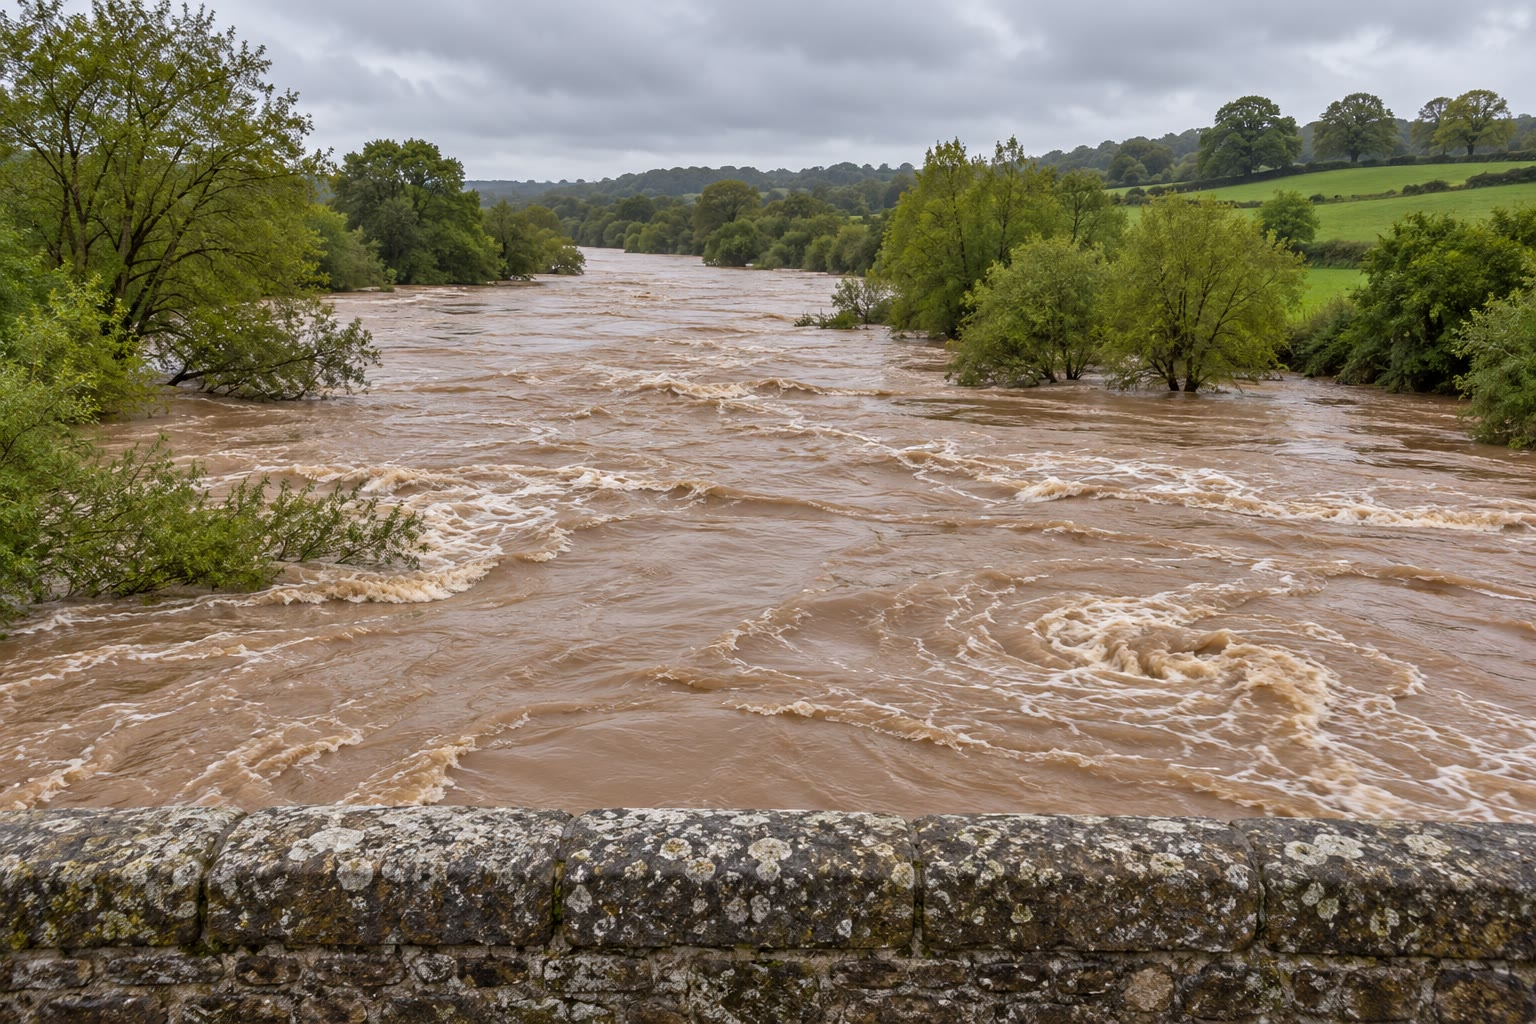
\includegraphics[height=5.1cm]{images/book3/ai/b1-muddy-river.jpg}\hfill
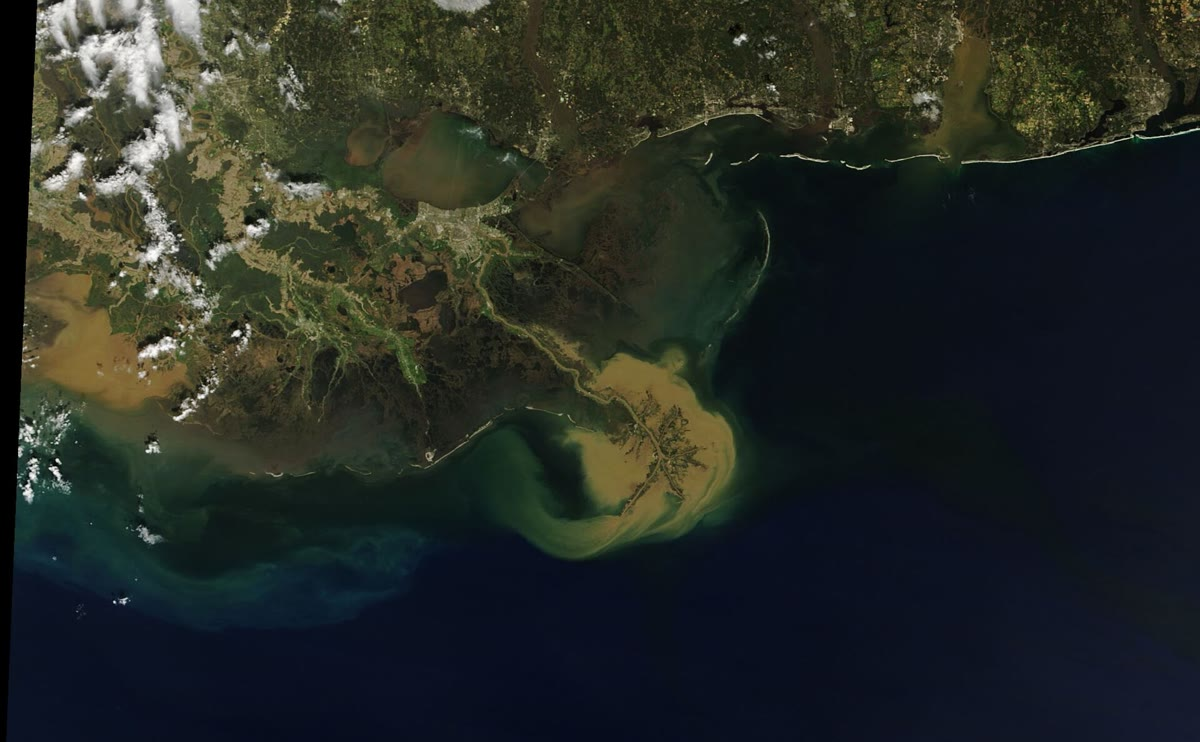
\includegraphics[height=5.1cm]{images/book3/b1-mississippi-plume.jpg}
\par\smallskip{\small À gauche~: une rivière en crue charrie une eau brune chargée de
sédiments (illustration IA). À droite~: le panache de crue du Mississippi se déversant
dans le golfe du Mexique autour de son delta, vu par l'instrument MODIS du
satellite Terra le 4~mars 2018~; la boue en suspension colore la mer de brun et de
vert, et le vent du sud-est pousse le panache vers le nord-ouest. Image du NASA Earth Observatory par Joshua Stevens, domaine public, via
Wikimedia Commons.}
\label{fig:b1:erosion-transport:plume}
\end{omfigure}
% ledger: commons:mississippi-plume

\emph{Les rivières du monde.} Avant toute influence humaine, les rivières du monde
transportaient environ \qty{14}{Gt} de sédiments en suspension par an vers l'océan
côtier, \qty{15.5}{Gt} avec la \omterm{def:b1:erosion-transport:load}{charge de fond}. Les humains ont changé les deux bouts du
voyage~: l'agriculture et la déforestation ont accru l'érosion des sols, ajoutant environ
\qty{2.3}{Gt} par an aux rivières, tandis que les réservoirs retiennent des sédiments~: les
grands piègent environ \qty{20}{\percent} du flux et les petits encore
\qty{6}{\percent}, et plus de \qty{100}{Gt} de sédiments reposent maintenant derrière des
barrages construits pour la plupart ces cinquante dernières années. L'effet net est une réduction~: le
flux actuel est d'environ \qty{12.6}{Gt} par an.
% ledger: syvitski:flux

\begin{dated}{2005}
Les chiffres du flux de sédiments en suspension, avant et après l'influence humaine,
proviennent d'un modèle mondial de sédiments fluviaux publié en 2005. Des barrages ont été
construits depuis.
\end{dated}
% ledger: syvitski:flux

La \omterm{def:b1:erosion-transport:load}{charge dissoute} est plus petite. Une compilation classique d'analyses de rivières, faite en
1963, estimait la matière dissoute que les rivières du monde livrent à la mer
à environ \qty{3.9}{Gt} par an, environ \qty{30}{\percent} du flux actuel en suspension,
à une concentration moyenne de \qty{120}{mg} par litre. Le bicarbonate en fait
près de la moitié, \qty{58}{mg.L^{-1}}, suivi du calcium, de la silice, du sulfate,
du chlorure et du sodium. Une partie ne vient pas de la roche~: une grande part du
bicarbonate porte du carbone tiré de l'air ou du sol, et une partie du
chlorure et du sodium vient du sel marin apporté par la pluie. Les rivières individuelles
s'écartent largement de ces moyennes.
% ledger: livingstone:world-dissolved, syvitski:flux

\emph{Le bilan sédimentaire d'un bassin.} Tous les grains érodés dans un bassin versant
n'atteignent pas son exutoire. Le sol lessivé d'un champ peut s'arrêter au pied de la
pente, le sable peut être stocké pendant des siècles dans la plaine d'inondation et les barres de la rivière,
et un réservoir peut retenir l'essentiel de ce qui y entre. La charge mesurée à
l'exutoire est le solde du bilan~: ce qui est érodé sur les versants et dans les
berges, moins ce qui est stocké en chemin, plus ce qui est repris aux anciens
stocks. Sur quelques décennies de jaugeage ce solde peut être très éloigné du
taux d'érosion à long terme, dans un sens ou dans l'autre, ce qui est une raison des
autres méthodes de la \cref{sec:b1:erosion-transport:denudation}.

\section{La vitesse de chute}\label{sec:b1:erosion-transport:settling}

Un grain est plus dense que l'eau et coule. Qu'une rivière puisse le transporter, et
où il se déposera, dépend d'abord de la vitesse à laquelle il coule.

\begin{definition}[Vitesse de chute]\label{def:b1:erosion-transport:settling}
La \emph{vitesse de chute}\index{vitesse de chute} $w_s$ d'un grain est la
vitesse constante à laquelle il tombe dans l'eau calme, quand la traînée de
l'eau équilibre son poids déjaugé, son poids moins la poussée d'Archimède de
l'eau qu'il déplace.
\end{definition}

Un grain lâché dans l'eau calme accélère jusqu'à ce que sa traînée, qui croît avec
sa vitesse, équilibre son poids déjaugé~; pour un grain de sable ou de silt cela
prend une petite fraction de seconde, donc la \omterm{def:b1:erosion-transport:settling}{vitesse de chute} est la vitesse à laquelle
il tombe presque tout le long du trajet. Avec les masses volumiques $\rho_s$ du grain
et $\rho$ de l'eau, posons $R = (\rho_s - \rho)/\rho$ pour la masse volumique
déjaugée relative.

\begin{proposition}[Chute de Stokes]\label{prop:b1:erosion-transport:stokes}
Une sphère de diamètre $d$ et de masse volumique $\rho_s$ tombant lentement dans de l'eau de masse
volumique $\rho$ et de viscosité dynamique $\mu$, sous la loi de Stokes, a pour \omterm{def:b1:erosion-transport:settling}{vitesse de
chute}
\[
  w_s = \frac{(\rho_s - \rho)\,g\,d^2}{18\,\mu} = \frac{R\,g\,d^2}{18\,\nu}.
\]
La loi vaut tant que le nombre de Reynolds du grain $w_s d/\nu$ est inférieur à environ 1,
c'est-à-dire pour des diamètres inférieurs à $d_1 = \left(18\,\nu^2/(R\,g)\right)^{1/3}$.
\end{proposition}

\begin{proof}
Le poids de la sphère est $\rho_s g\,\pi d^3/6$ et la poussée d'Archimède
$\rho g\,\pi d^3/6$, donc son poids déjaugé est $(\rho_s - \rho)\,g\,\pi d^3/6$.
À la \omterm{def:b1:erosion-transport:settling}{vitesse de chute} il égale la traînée $3\pi\mu d\,w_s$~:
\[
  (\rho_s - \rho)\,g\,\frac{\pi d^3}{6} = 3\pi\mu d\,w_s
  \quad\Longrightarrow\quad
  w_s = \frac{(\rho_s - \rho)\,g\,d^2}{18\,\mu},
\]
et en divisant le numérateur et le dénominateur par $\rho$ on obtient la seconde forme.
Le nombre de Reynolds de cette vitesse est $R g d^3/(18\nu^2)$, qui vaut 1 pour
$d = d_1$ et croît comme $d^3$.
\end{proof}

Pour le quartz, de masse volumique \qty{2650}{kg.m^{-3}}, dans de l'eau à \qty{20}{\celsius},
de masse volumique \qty{998.2}{kg.m^{-3}} et de viscosité \qty{1.0016}{mPa.s}~: $R =
1.65$, $\nu = \qty{1.003e-6}{m^2.s^{-1}}$, et avec $g =
\qty{9.81}{m.s^{-2}}$ la limite est $d_1 = \qty{0.104}{mm}$, un sable fin. En dessous,
la loi de Stokes donne les \omterm{def:b1:erosion-transport:settling}{vitesses de chute} du silt et de l'argile~: un grain de silt
de \qty{10}{\micro m} coule à \qty{9.0e-5}{m.s^{-1}}, \qty{1}{m} en environ
trois heures~; une particule d'argile de \qty{2}{\micro m} à
\qty{3.6e-6}{m.s^{-1}}, \qty{1}{m} en \num{3.2}~jours. Les particules d'argile naturelles sont
des paillettes, non des sphères, et coulent plus lentement encore. Une eau profonde de \qty{5}{m}, parfaitement
calme, mettrait seize jours à s'éclaircir d'une telle argile~; une rivière qui coule, dont les
tourbillons la remettent sans cesse en suspension, ne s'éclaircit jamais, c'est pourquoi la boue la plus fine voyage
jusqu'à la mer.
% ledger: hom:quartz, nist:water, const:gn

Au-dessus de $d_1$ la traînée croît plus vite que proportionnellement à la vitesse~: l'eau
qui passe devant le grain se sépare derrière lui en un sillage, et aux grands nombres de Reynolds
la traînée est proportionnelle au carré de la vitesse. Des expériences sur
des grains naturels sont résumées en une seule formule qui raccorde les deux régimes.

\begin{proposition}[Loi de chute combinée]\label{prop:b1:erosion-transport:combined}
La \omterm{def:b1:erosion-transport:settling}{vitesse de chute} de grains naturels de diamètre de tamis $d$ est, pour toutes les
tailles,
\[
  w_s = \frac{R\,g\,d^2}{C_1\,\nu + \sqrt{0.75\,C_2\,R\,g\,d^3}},
\]
avec $C_1 = 18$ et $C_2 = 1.0$.
\end{proposition}
\admitted
% ledger: fc:settling

La loi est due à Ferguson et Church, qui l'ont ajustée sur des \omterm{def:b1:erosion-transport:settling}{vitesses de chute}
mesurées de sables naturels. Pour les petits grains la racine carrée est
négligeable et elle se réduit à la loi de Stokes~; pour les grands grains le premier terme du
dénominateur est négligeable et $w_s \to \sqrt{4 R g d/(3 C_2)}$, qui ne croît
que comme la racine carrée de la taille. Les constantes dépendent de la forme des
grains~: $C_2 = 0.4$ décrit des sphères lisses, des valeurs plus grandes des grains plus
anguleux, qui subissent davantage de traînée. Les deux lois divergent au-dessus de
\qty{0.1}{mm}. Pour un grain de \qty{1}{mm} la loi combinée donne
\qty{0.126}{m.s^{-1}}, sept fois moins que la loi de Stokes~; pour un galet de
\qty{10}{mm}, \qty{0.46}{m.s^{-1}} contre un \qty{90}{m.s^{-1}} dénué de sens
(diagramme ci-dessous).
% ledger: fc:settling

\begin{omfigure}
\begin{tikzpicture}[font=\small]
% settling velocity of quartz grains in water at 20 C (figdata/bachelor-1/settling.py)
\begin{axis}[width=11cm, xmode=log, ymode=log, xmin=0.001, xmax=10, ymin=1e-8, ymax=10, height=8cm,
    xlabel={diamètre du grain $d$ (\si{mm})}, ylabel={vitesse de chute (\si{m.s^{-1}})},
    ytick={1e-8,1e-6,1e-4,1e-2,1},
    legend style={at={(0.03,0.97)}, anchor=north west, font=\footnotesize}, legend cell align=left,
    grid=major, grid style={black!10}]
  \addplot[omDef, thick, dashed] table[x=d_mm, y=w_stokes] {figdata/out/bachelor-1-settling-curves.dat};
  \addplot[omThm, very thick] table[x=d_mm, y=w_fc] {figdata/out/bachelor-1-settling-curves.dat};
  \legend{loi de Stokes, loi combinée (grains naturels)}
  \draw[black!55, densely dotted] (axis cs:0.1037,1e-7) -- (axis cs:0.1037,10);
  \node[font=\scriptsize, anchor=west, align=left, black!75] at (axis cs:0.115,1e-6) {nombre de Reynolds\\ du grain $= 1$};
  \node[font=\scriptsize, black!70] at (axis cs:0.002,3e-8) {argile};
  \node[font=\scriptsize, black!70] at (axis cs:0.016,3e-8) {silt};
  \node[font=\scriptsize, black!70] at (axis cs:0.35,3e-8) {sable};
  \node[font=\scriptsize, black!70] at (axis cs:4.5,3e-8) {gravier};
  \draw[black!40] (axis cs:0.0039,1e-8) -- (axis cs:0.0039,1e-7);
  \draw[black!40] (axis cs:0.0625,1e-8) -- (axis cs:0.0625,1e-7);
  \draw[black!40] (axis cs:2,1e-8) -- (axis cs:2,1e-7);
\end{axis}
\end{tikzpicture}

{\small \omterm{def:b1:erosion-transport:settling}{Vitesse de chute} de grains de quartz dans l'eau à \qty{20}{\celsius}
en fonction de leur diamètre, les deux en échelles logarithmiques~: loi de Stokes et
loi combinée des grains naturels, calculées. Sur ces échelles la loi de Stokes est une
droite de pente 2. Les deux s'accordent pour le silt et l'argile~; au-dessus d'environ
\qty{0.1}{mm}, où le nombre de Reynolds du grain dépasse 1, la traînée du sillage
ralentit les grains grossiers. Les repères en bas marquent les limites des
classes granulométriques, à \qty{3.9}{\micro m} ($1/256$~mm), \qty{62.5}{\micro m}
($1/16$~mm) et \qty{2}{mm}.}
\label{fig:b1:erosion-transport:settling}
\end{omfigure}
% ledger: fc:settling, usgs:wentworth-phi

Sur l'étendue du diagramme, de l'argile la plus fine à un gravier grossier, la
\omterm{def:b1:erosion-transport:settling}{vitesse de chute} couvre huit ordres de grandeur. C'est la première raison pour laquelle les
rivières trient leurs sédiments~: un courant qui faiblit lâche son gravier d'un coup, son
sable en quelques mètres, son silt en quelques kilomètres, et porte son argile jusqu'à un
lac ou à la mer. Les classes granulométriques et le tri des sédiments sont
le sujet du chapitre suivant (\cref{ch:b1:clastic-sediments}).

\section{Seuil de mise en mouvement et diagramme de Hjulström}\label{sec:b1:erosion-transport:threshold}

Un grain au repos sur le lit d'une rivière est mis en mouvement par la force de l'eau
qui coule sur lui. Cette force se mesure par une contrainte.

\begin{definition}[Contrainte de cisaillement au fond, vitesse de cisaillement]\label{def:b1:erosion-transport:bed-shear}
La \emph{contrainte de cisaillement au fond}\index{contrainte de cisaillement au fond} $\tau_b$ d'un écoulement est la
force par unité d'aire qu'il exerce sur son lit, parallèlement au lit, dans la
direction de l'écoulement. La vitesse de cisaillement est $u_* = \sqrt{\tau_b/\rho}$, une
vitesse qui mesure la même contrainte.
\end{definition}

La \omterm{def:b1:erosion-transport:bed-shear}{contrainte de cisaillement au fond} ne se lit pas sur un courantomètre, mais dans un écoulement
permanent elle découle d'un bilan de forces.

\begin{proposition}[Produit profondeur--pente]\label{prop:b1:erosion-transport:depth-slope}
Dans un écoulement permanent et uniforme de profondeur $h$ le long d'un large chenal de faible pente $S$,
la \omterm{def:b1:erosion-transport:bed-shear}{contrainte de cisaillement au fond} est
\[
  \tau_b = \rho\,g\,h\,S .
\]
\end{proposition}

\begin{proof}
Considérons l'eau au-dessus d'un morceau de fond de longueur $L$ le long de l'écoulement et de
largeur unité, le chenal étant si large que ses berges peuvent être ignorées. L'écoulement
est permanent et uniforme, donc cette eau n'accélère pas et les forces sur elle
s'équilibrent. Les forces de pression sur ses faces amont et aval sont égales et
opposées, puisque la profondeur est la même des deux côtés. Le long de l'écoulement il reste la
composante du poids, $\rho g h L \sin\beta$, où $\beta$ est l'angle du
fond, et le frottement du fond, $\tau_b L$, qui s'y oppose. D'où $\tau_b
= \rho g h \sin\beta$, et pour un petit angle $\sin\beta \approx \tan\beta = S$.
\end{proof}

Une rivière profonde de \qty{2}{m} sur une pente de \num{0.001}, un mètre de chute par
kilomètre, a $\tau_b = 998.2 \times 9.81 \times 2 \times 0.001 =
\qty{19.6}{Pa}$, et une vitesse de cisaillement de \qty{0.140}{m.s^{-1}}. Dans un chenal
qui n'est pas large, les berges prennent leur part du frottement, et la profondeur est
remplacée par le rayon hydraulique, l'aire de la section divisée par son périmètre
mouillé (\cref{exo:b1:erosion-transport:5}).

\emph{Les forces sur un grain.} L'écoulement pousse un grain du fond par sa traînée et
le soulève par l'écoulement plus rapide au-dessus de lui (l'encart de la première figure de ce
chapitre). Les deux forces agissent sur l'aire du grain, donc elles varient comme $\tau_b
d^2$~; le grain résiste par son poids déjaugé, qui varie comme
$(\rho_s - \rho) g d^3$. Le rapport des deux est la mesure naturelle de la
force de l'écoulement pour un grain donné.

\begin{definition}[Paramètre de Shields, seuil de mise en mouvement]\label{def:b1:erosion-transport:threshold}
Le \emph{paramètre de Shields}\index{parametre de Shields@paramètre de Shields} d'un écoulement de \omterm{def:b1:erosion-transport:bed-shear}{contrainte de cisaillement au fond}
$\tau_b$ sur des grains de diamètre $d$ et de masse volumique $\rho_s$ est
\[
  \theta = \frac{\tau_b}{(\rho_s - \rho)\,g\,d}.
\]
Le \emph{seuil de mise en mouvement}\index{seuil de mise en mouvement} des grains est la
\omterm{def:b1:erosion-transport:bed-shear}{contrainte de cisaillement au fond}, ou la valeur $\theta_c$ du paramètre de Shields, à laquelle
ils commencent à bouger.
\end{definition}
% ledger: hecras:thresholds

La valeur critique $\theta_c$ est mesurée en canal, et les mesures tombent
sur une seule courbe quand on les trace en fonction d'une taille de grain sans dimension qui
combine le grain et le fluide.

\begin{proposition}[Courbe de seuil de Soulsby et Whitehouse]\label{prop:b1:erosion-transport:soulsby}
Pour des grains de diamètre $d$ sur un fond plat, avec
$D_* = d\,\left(R\,g/\nu^2\right)^{1/3}$, le \omterm{def:b1:erosion-transport:threshold}{paramètre de Shields} critique est
\[
  \theta_c = \frac{0.3}{1 + 1.2\,D_*} + 0.055\left(1 - e^{-0.02\,D_*}\right),
\]
et la contrainte de cisaillement critique au fond est $\tau_c = \theta_c\,(\rho_s - \rho)\,g\,d$.
\end{proposition}
\admitted
% ledger: hecras:thresholds

Pour les gros grains $\theta_c$ tend vers \num{0.055}~: le gravier bouge quand la \omterm{def:b1:erosion-transport:bed-shear}{contrainte de
cisaillement au fond} atteint environ un vingtième du poids déjaugé d'une couche de
grains épaisse d'un diamètre, par unité d'aire. Les formules de transport sédimentaire qui
utilisent un seuil constant prennent des valeurs de \num{0.03} à \num{0.047}, cette
dernière dans la formule classique de \omterm{def:b1:erosion-transport:load}{charge de fond} de Meyer-Peter et Müller. Pour le sable fin $\theta_c$ remonte, à
\num{0.077} à \qty{0.1}{mm}~: les petits grains se trouvent dans la couche lente et visqueuse
d'eau proche du fond et sont abrités par leurs voisins. Le minimum,
\num{0.030}, tombe vers \qty{0.7}{mm}. En pascals le seuil croît toujours
avec la taille (diagramme ci-dessous)~: \qty{0.13}{Pa} pour un sable de \qty{0.1}{mm},
\qty{0.51}{Pa} à \qty{1}{mm}, \qty{9.0}{Pa} à \qty{10}{mm}, \qty{57}{Pa} pour un
galet de \qty{64}{mm}.
% ledger: hecras:thresholds

\begin{omfigure}
\begin{tikzpicture}[font=\small]
% threshold of motion of quartz grains in water at 20 C (figdata/bachelor-1/threshold.py, Soulsby and Whitehouse)
\begin{axis}[name=a, width=6.9cm, height=6cm, xmode=log, xmin=0.0625, xmax=100, ymin=0, ymax=0.12,
    xlabel={diamètre du grain $d$ (\si{mm})}, ylabel={paramètre de Shields critique $\theta_c$},
    yticklabel style={/pgf/number format/fixed, /pgf/number format/precision=2},
    grid=major, grid style={black!10}, title={\footnotesize (a) sans dimension}]
  \addplot[omThm, very thick] table[x=d_mm, y=theta] {figdata/out/bachelor-1-threshold-shields.dat};
  \draw[black!50, dashed] (axis cs:0.0625,0.055) -- (axis cs:100,0.055) node[pos=0.7, above, font=\scriptsize, black!70] {$0.055$};
\end{axis}
\begin{axis}[at={(a.east)}, anchor=west, xshift=2.0cm, width=6.9cm, height=6cm, xmode=log, ymode=log,
    xmin=0.0625, xmax=100, ymin=0.05, ymax=200,
    xlabel={diamètre du grain $d$ (\si{mm})}, ylabel={contrainte de cisaillement critique au fond $\tau_c$ (\si{Pa})},
    grid=major, grid style={black!10}, title={\footnotesize (b) en pascals}]
  \addplot[omDef, very thick] table[x=d_mm, y=tau_cr] {figdata/out/bachelor-1-threshold-shields.dat};
\end{axis}
\end{tikzpicture}

{\small Le \omterm{def:b1:erosion-transport:threshold}{seuil de mise en mouvement} de grains de quartz dans l'eau à
\qty{20}{\celsius}, d'après la courbe de Soulsby et Whitehouse, calculé de la limite du sable fin
(\qty{0.0625}{mm}) à la taille d'un galet. (a)~Le \omterm{def:b1:erosion-transport:threshold}{paramètre de Shields} critique
est presque constant pour le gravier et monte pour le sable fin. (b)~La contrainte de
cisaillement critique au fond croît presque proportionnellement au diamètre pour le gravier.}
\label{fig:b1:erosion-transport:threshold}
\end{omfigure}
% ledger: hecras:thresholds

\begin{example}[Ce que la rivière déplace]\label{ex:b1:erosion-transport:river}
Dans la rivière profonde de \qty{2}{m} sur une pente de \num{0.001}, $\tau_b =
\qty{19.6}{Pa}$. Pour des grains de \qty{20}{mm}, $\theta = 19.6/(1651.8 \times
9.81 \times 0.020) = 0.060$, juste au-dessus de leur seuil de \num{0.055}~: ils
bougent. Pour des grains de \qty{40}{mm}, $\theta = 0.030$, la moitié du seuil~: ils
restent. La rivière déplace son lit jusqu'au gravier grossier~; pour du sable de \qty{1}{mm},
$\theta = 1.21$, près de quarante fois le seuil de \num{0.031}.
\end{example}

\emph{Vers la suspension.} Une fois en mouvement, un grain saute le long du fond ou est repris
dans l'écoulement, selon que les tourbillons, dont les vitesses sont de l'ordre
de la vitesse de cisaillement, peuvent le maintenir contre sa chute.

\begin{proposition}[Critère de suspension]\label{prop:b1:erosion-transport:suspension}
Un grain de \omterm{def:b1:erosion-transport:settling}{vitesse de chute} $w_s$ ne peut rester en suspension dans un écoulement turbulent
que si certains tourbillons montent plus vite qu'il ne coule. Les vitesses ascendantes des
tourbillons étant de l'ordre de la vitesse de cisaillement $u_*$, la suspension commence quand
$u_*$ approche $w_s$ et est pleinement développée quand $u_*$ la dépasse~; ce
chapitre prend $u_* = w_s$ comme limite de la suspension.
\end{proposition}
\admitted
% ledger: bagnold:suspension

Dans la rivière de l'exemple, $u_* = \qty{0.140}{m.s^{-1}}$, que la loi combinée
de chute donne à des grains de \qty{1.16}{mm}~: le sable plus fin qu'environ un
millimètre voyage en suspension, le sable plus grossier et le gravier comme \omterm{def:b1:erosion-transport:load}{charge de fond}.
L'argument remonte à Bagnold, qui nota que des grains de \qty{0.1}{mm} ou
moins sont entièrement en suspension dès qu'ils bougent, alors que des grains plus gros que
\qty{1}{mm} demandent une \omterm{def:b1:erosion-transport:bed-shear}{contrainte de cisaillement au fond} de bien des fois leur seuil. Quand
la crue décroît et que $u_*$ baisse, le sable grossier retombe d'abord sur le fond.

\emph{De la contrainte à la vitesse moyenne.} Ce qui se mesure ou s'estime facilement dans
une rivière est sa vitesse moyenne. Dans un écoulement turbulent sur un fond rugueux
de grains de diamètre $d$, un large chenal de profondeur $h$ a pour vitesse moyenne
$U = u_*\left(6.25 + 5.75\log_{10}(h/d)\right)$, une loi établie par Keulegan
en 1938 à partir des expériences de Nikuradse et de Bazin, donc le \omterm{def:b1:erosion-transport:threshold}{seuil de mise en mouvement}
correspond à la vitesse moyenne critique
\[
  U_c = \left(6.25 + 5.75\,\log_{10}\frac{h}{d}\right)\sqrt{\theta_c\,R\,g\,d},
\]
et la limite de suspension, $u_* = w_s$, à $U_s = \left(6.25 +
5.75\log_{10}(h/d)\right) w_s$. Les deux dépendent de la profondeur, mais seulement par un
logarithme.
% ledger: keulegan:mean-velocity, bagnold:suspension

Les vitesses de seuil appartiennent donc à une profondeur et à un jeu de lois~:
calculées pour une autre profondeur, ou lues dans d'autres mesures, elles sortent
différentes. Tracées en fonction de la taille des grains, leur forme est robuste mais leurs
valeurs ne le sont pas, et la \omterm{def:b1:erosion-transport:bed-shear}{contrainte de cisaillement au fond}, qui ne dépend pas de la profondeur de
la même façon, est la meilleure mesure de ce qu'un écoulement peut faire. Les vitesses sont
pourtant plus intuitives, et la façon classique de les représenter est un diagramme.

\begin{definition}[Diagramme de Hjulström]\label{def:b1:erosion-transport:hjulstrom}
Un \emph{diagramme de Hjulström}\index{diagramme de Hjulstrom@diagramme de Hjulström} trace la vitesse moyenne
d'un écoulement en fonction du diamètre des grains, en échelles logarithmiques, et divise
le plan en domaines où les grains au repos sont érodés, les grains déjà
en mouvement sont maintenus en transport, et les grains en mouvement sont déposés.
\end{definition}
% ledger: hjulstrom:curve

\begin{omfigure}
\begin{tikzpicture}[font=\small]
% Hjulstrom-type diagram for a flow 1 m deep (figdata/bachelor-1/threshold.py); the hatched
% cohesive field is schematic (its lower edge, 30 cm/s, is not computed)
\begin{axis}[width=12cm, height=8.4cm, xmode=log, ymode=log, xmin=0.001, xmax=100, ymin=0.1, ymax=3000,
    xlabel={diamètre du grain $d$ (\si{mm})}, ylabel={vitesse moyenne de l'écoulement (\si{cm.s^{-1}})},
    unbounded coords=jump, grid=major, grid style={black!10}]
  \addplot[draw=none, name path=dep] table[x=d_mm, y=u_dep] {figdata/out/bachelor-1-threshold-hjul.dat};
  \addplot[draw=none, name path=bot] coordinates {(0.001,0.1) (100,0.1)};
  \addplot[fill=omDef!14, draw=none] fill between[of=dep and bot];
  \fill[pattern=north east lines, pattern color=omThm!45] (axis cs:0.001,30) rectangle (axis cs:0.0625,3000);
  \addplot[omThm, very thick] table[x=d_mm, y=u_cr] {figdata/out/bachelor-1-threshold-hjul.dat};
  \addplot[omDef, very thick, dashed] table[x=d_mm, y=u_s] {figdata/out/bachelor-1-threshold-hjul.dat};
  \node[font=\footnotesize, fill=white, fill opacity=0.85, text opacity=1, align=center] at (axis cs:0.5,1500) {\textbf{érosion}~: grains emportés en suspension};
  \node[font=\footnotesize, fill=white, fill opacity=0.85, text opacity=1, align=center] at (axis cs:22,330) {\textbf{charge de fond}};
  \node[font=\footnotesize, fill=white, fill opacity=0.85, text opacity=1, align=center, anchor=west] at (axis cs:0.00115,2.5) {\textbf{transport}~:\\ les grains déjà\\ en mouvement restent\\ en suspension};
  \node[font=\footnotesize, fill=white, fill opacity=0.85, text opacity=1, align=center] at (axis cs:3,0.6) {\textbf{dépôt}};
  \node[font=\footnotesize, fill=white, fill opacity=0.85, text opacity=1, align=center] at (axis cs:0.008,300) {boue cohésive~:\\ seuil fixé par\\ le compactage};
  \node[font=\scriptsize, omThm, anchor=north, rotate=12] at (axis cs:6,80) {seuil de mise en mouvement};
  \node[font=\scriptsize, omDef, anchor=north west, rotate=57] at (axis cs:0.028,0.95) {limite de suspension};
  \draw (rel axis cs:0,0) -- (rel axis cs:1,0);
\end{axis}
\end{tikzpicture}

{\small Un diagramme de type Hjulström pour des grains de quartz dans une eau
profonde de \qty{1}{m} à \qty{20}{\celsius}, calculé~: le \omterm{def:b1:erosion-transport:threshold}{seuil de mise en mouvement} (trait plein)
d'après la courbe de Soulsby et Whitehouse, la limite de suspension (tirets) d'après
la loi de chute combinée, tous deux transformés en vitesses moyennes par la loi de Keulegan. Au-dessus de la courbe pleine, les grains
au repos sont érodés~; sous la plus basse des deux courbes (grisée), les grains en mouvement
sont déposés. Les grains plus fins que \qty{0.13}{mm} passent en suspension dès qu'ils
bougent~; les plus gros voyagent d'abord comme \omterm{def:b1:erosion-transport:load}{charge de fond}. Le calcul ne vaut que
pour des grains meubles~: le domaine hachuré du silt et de l'argile cohésifs est schématique.}
\label{fig:b1:erosion-transport:hjulstrom}
\end{omfigure}
% ledger: hecras:thresholds, fc:settling, bagnold:suspension, keulegan:mean-velocity

\emph{Lire le diagramme.} Trois traits portent la géologie. D'abord, les
grains les plus faciles à éroder sont les sables fins, entre environ \num{0.06} et
\qty{0.2}{mm}, qu'un courant de \qtyrange{31}{34}{cm.s^{-1}} met en mouvement dans
une eau profonde de \qty{1}{m}~; les grains plus gros demandent davantage, jusqu'à environ
\qty{3}{m.s^{-1}} pour un galet de \qty{64}{mm}. Ensuite, le silt et l'argile, bien
que plus légers, sont plus difficiles à éroder que le sable fin une fois déposés~:
leurs particules collent ensemble, et une boue compactée résiste à un courant qui
balaierait le sable. Le calcul pour des grains meubles ne peut le voir, et
les vitesses d'érosion mesurées des boues varient avec leur compactage et leur teneur en
eau, d'où le domaine hachuré. Enfin, l'écart entre érosion et
dépôt s'ouvre largement pour les grains fins~: une particule d'argile demande un courant
fort pour être arrachée à un fond vaseux, mais une fois dans l'eau elle y reste dans
l'écoulement le plus doux, ce qui est toute l'histoire de la crue brune et du
panache dans la mer.
% ledger: hjulstrom:curve, hecras:thresholds, keulegan:mean-velocity

\begin{history}[Deux études des années 1930]
En 1935 Filip Hjulström, de l'Institut géographique d'Uppsala, publia une
longue étude du travail de la rivière Fyris, dans le centre de la Suède, qui contenait
le diagramme qui porte son nom~: vitesses d'érosion et de dépôt en fonction de
la taille des grains, en échelles logarithmiques. À la différence des courbes antérieures, sa courbe d'érosion avait
un minimum, entre environ \num{0.1} et \qty{0.5}{mm}~: le sable fin meuble est le
plus facile à éroder, alors que le sable plus grossier et le gravier, et aussi le silt et l'argile, qui
sont cohésifs, demandent des courants plus forts. Un an plus tard, en 1936, l'ingénieur A.~Shields,
dans la thèse qu'il soutint à la Technische Hochschule de Berlin, traça
le \omterm{def:b1:erosion-transport:threshold}{seuil de mise en mouvement} comme un rapport de forces, le paramètre qui porte maintenant
son nom, en fonction d'une taille de grain sans dimension. Les vitesses de Hjulström ignorent la
profondeur de l'écoulement~; l'approche sans dimension de Shields non, et elle sous-tend
les formules de seuil utilisées aujourd'hui, comme celle qui est derrière les diagrammes de ce
chapitre.
\end{history}
% ledger: hjulstrom:curve, shields:1936, hecras:thresholds

\section{Les taux de dénudation}\label{sec:b1:erosion-transport:denudation}

Les charges d'une rivière, additionnées sur son bassin, mesurent la vitesse à laquelle le bassin
est usé.

\begin{definition}[Taux de dénudation]\label{def:b1:erosion-transport:denudation}
Le \emph{taux de dénudation}\index{taux de denudation@taux de dénudation} $D$ d'une région est la vitesse moyenne
à laquelle l'enlèvement de matière, sous forme de grains solides et en solution, abaisse
sa surface, exprimée comme l'épaisseur équivalente de roche fraîche par unité de
temps, en mètres par million d'années (\unit{m/\Ma}, la même chose que des millimètres par
millier d'années). La masse enlevée par unité d'aire et de temps, en tonnes par kilomètre
carré et par an, est le flux sédimentaire spécifique.
\end{definition}

\begin{proposition}[La dénudation d'après les charges fluviales]\label{prop:b1:erosion-transport:denudation}
Si un bassin d'aire $A$ perd, par son exutoire, les masses annuelles $F_s$ de
\omterm{def:b1:erosion-transport:load}{charge en suspension}, $F_b$ de \omterm{def:b1:erosion-transport:load}{charge de fond} et $F_d$ de \omterm{def:b1:erosion-transport:load}{charge dissoute} issue de ses
roches, et si rien n'est stocké en chemin, son \omterm{def:b1:erosion-transport:denudation}{taux de dénudation} est
\[
  D = \frac{F_s + F_b + F_d}{\rho_r\,A},
\]
avec $\rho_r$ la masse volumique de la roche fraîche. Pour $\rho_r =
\qty{2700}{kg.m^{-3}}$, un flux spécifique de \qty{100}{t.km^{-2}.\year^{-1}}
correspond à \qty{37}{m/\Ma}.
\end{proposition}

\begin{proof}
La masse perdue par unité d'aire et de temps est $(F_s + F_b + F_d)/A$~; divisée par la
masse volumique de la roche elle devient l'épaisseur de roche perdue par unité de temps. Pour
la conversion, \qty{100}{t.km^{-2}.\year^{-1}} fait
$\qty{1e5}{kg}/\qty{1e6}{m^2} = \qty{0.1}{kg.m^{-2}}$ par an, soit
$0.1/2700 = \qty{3.7e-5}{m}$ par an, \qty{37}{m} par million d'années.
\end{proof}

La \omterm{def:b1:erosion-transport:load}{charge dissoute} ne compte que pour la part qui vient de la roche, non de
l'air~: le carbone du bicarbonate de l'altération des silicates est pris à
l'atmosphère, et seuls les cations et la silice sont de la roche. La part chimique de
la dénudation n'est pas petite. Là où le climat est chaud et humide et le relief bas,
elle peut approcher ou dépasser la part mécanique, alors que dans les montagnes raides
la part mécanique domine.

\emph{Trois horloges.} Le \omterm{def:b1:erosion-transport:denudation}{taux de dénudation} peut se mesurer sur trois durées très
différentes. Les charges des rivières intègrent des années à des décennies, et sont à
la merci des quelques crues qui ont eu lieu, ou non, pendant les
mesures. Le sédiment piégé dans un réservoir ou un lac, mesuré en levant
son fond, intègre les décennies à un siècle de sa vie. La
troisième horloge est écrite dans les grains eux-mêmes, par les rayons cosmiques.

\begin{proposition}[Nucléides cosmogéniques et érosion]\label{prop:b1:erosion-transport:cosmogenic}
Supposons qu'un nucléide soit produit dans une roche par les rayons cosmiques au taux
$P(z) = P_0\,e^{-\rho z/\Lambda}$ par unité de masse, décroissant exponentiellement avec
la profondeur $z$ ($\rho$ la masse volumique de la roche, $\Lambda$ une constante, la
longueur d'atténuation exprimée comme une masse par unité d'aire), et que la surface soit
abaissée au taux constant $\varepsilon$. En négligeant la décroissance radioactive, un grain
qui atteint la surface porte la concentration
\[
  N = \frac{P_0\,\Lambda}{\rho\,\varepsilon}.
\]
\end{proposition}

\begin{proof}
Relativement à la surface, qui descend à la vitesse $\varepsilon$, un grain
monte à la vitesse $\varepsilon$, donc il passe le temps $\mathrm dz/\varepsilon$
dans une couche d'épaisseur $\mathrm dz$ à la profondeur $z$, et y gagne la
concentration $P(z)\,\mathrm dz/\varepsilon$. En remontant de grande profondeur, il
atteint la surface avec
\[
  N = \frac{1}{\varepsilon}\int_0^{\infty} P_0\,e^{-\rho z/\Lambda}\,\mathrm dz
  = \frac{P_0}{\varepsilon}\,\frac{\Lambda}{\rho}. \qedhere
\]
\end{proof}

La concentration est inversement proportionnelle au taux d'érosion~: une surface qui
s'érode lentement garde chaque grain près de la surface longtemps et le charge
de nucléides. Le taux qu'elle donne est moyenné sur le temps mis à éroder les
quelques mètres où la production est concentrée, soit d'environ
mille à un million d'années, selon le taux. Négliger la décroissance est
justifié quand ce temps est court devant la vie du nucléide~; quand
l'érosion est très lente, la décroissance est incluse et la formule devient un peu
plus longue.
% ledger: portenga:method

\begin{inthelab}[Le béryllium-10 dans le sable de rivière]
Le nucléide habituel est le béryllium-10, par ailleurs exceptionnellement rare à la
surface de la Terre, fait par les rayons cosmiques dans le quartz des quelques premiers mètres
de roche. Pour mesurer
le \omterm{def:b1:erosion-transport:denudation}{taux de dénudation} d'un bassin entier, les géochimistes collectent du sable sur le lit de
sa rivière près de l'exutoire, en supposant que la rivière mélange des grains de
tous les versants du bassin proportionnellement à la vitesse à laquelle chacun est érodé. Au
laboratoire, le quartz est séparé des autres minéraux et nettoyé dans des
acides qui en ôtent le béryllium formé dans l'air et ramené par la pluie~; il est ensuite
dissous, une quantité connue de béryllium ordinaire est ajoutée, et le béryllium
est extrait. Ses isotopes sont comptés un atome à la fois avec un spectromètre de
masse à accélérateur, qui peut trouver les rares atomes de béryllium-10 parmi un vaste
excès de l'isotope ordinaire.
\end{inthelab}
% ledger: portenga:method

\emph{Quels sont les taux.} Une compilation de \num{1599} telles mesures,
publiée en 2011, a trouvé que les \omterm{def:b1:geological-maps:geological-map}{affleurements} nus de roche s'abaissent lentement~: de
\qty{12}{m/\Ma} en moyenne, avec une médiane de \qty{5.4}{m/\Ma} (450 \omterm{def:b1:geological-maps:geological-map}{affleurements}).
La roche sédimentaire s'use plus vite, \qty{20}{m/\Ma} en moyenne, que la
métamorphique, \qty{11}{m/\Ma}, et l'ignée, \qty{8.7}{m/\Ma}. Des bassins versants
entiers perdent bien davantage, \qty{218}{m/\Ma} en moyenne avec une médiane de
\qty{54}{m/\Ma} (\num{1149} bassins)~: leurs pentes raides, glissements de terrain et
chenaux de rivière s'érodent bien plus vite que leurs sommets nus, et quelques bassins très rapides
élèvent la moyenne à quatre fois la médiane. La pente moyenne d'un bassin est le
meilleur prédicteur unique de son taux. Les bassins dans des régions sismiquement actives, où
les montagnes se soulèvent, font en moyenne \qty{367}{m/\Ma}, contre \qty{182}{m/\Ma} dans les
régions calmes~; les bassins polaires, rabotés par les glaciers, \qty{537}{m/\Ma}~; les bassins arides
\qty{100}{m/\Ma}.
% ledger: portenga:rates

\emph{L'\omterm{def:b1:isostasy-gravity:isostasy}{isostasie} ralentit l'abaissement.} Enlever de la roche d'une région en \omterm{def:b1:isostasy-gravity:isostasy}{isostasie}
allège ses colonnes, et la \omterm{def:b1:layered-earth:layers}{croûte} se soulève pour rétablir l'équilibre. Avec $\rho_c
= \qty{2700}{kg.m^{-3}}$ et $\rho_m = \qty{3300}{kg.m^{-3}}$
(\cref{ch:b1:isostasy-gravity}), la formule du rebond rappelée au début du
chapitre donne un abaissement de seulement $1 - 2700/3300 = 0.18$ de l'épaisseur
enlevée~: pour abaisser la surface moyenne d'une région de \qty{1}{m}, l'érosion doit
enlever \qty{5.5}{m} de roche. Le temps pour user une chaîne de montagnes est donc
plus de cinq fois ce que suggère sa hauteur divisée par son \omterm{def:b1:erosion-transport:denudation}{taux de dénudation},
et les roches maintenant à la surface de vieilles chaînes arasées se trouvaient autrefois à de nombreux
kilomètres de profondeur. Et comme le rebond suit l'épaisseur moyenne enlevée,
non sa répartition, une chaîne dont les vallées sont creusées profondément tandis que les sommets sont
à peine touchés se soulève dans son ensemble~: ses sommets montent, bien que rien n'y ait
été ajouté (\cref{exo:b1:erosion-transport:11}).

\emph{Les taux changent.} Un \omterm{def:b1:erosion-transport:denudation}{taux de dénudation} mesuré aujourd'hui n'est pas une constante du
paysage. À mesure que le relief et les pentes diminuent, le taux aussi, et une
vieille chaîne abaissée s'use toujours plus lentement~; à l'inverse, une chaîne en cours de
soulèvement, ou un climat qui change, l'élève. Un temps calculé à partir du taux
d'aujourd'hui est une première estimation, non une prédiction.

\section{Exercices}

\begin{exercise}[$\star$]\label{exo:b1:erosion-transport:1}
Une rivière a un débit moyen de \qty{500}{m^3.s^{-1}} et transporte, en moyenne
pondérée par le débit, \qty{0.4}{g} de sédiment en suspension par litre. Calculer son
flux en suspension en kilogrammes par seconde et en millions de tonnes par an (prendre une
année de \num{365.25}~jours).
\end{exercise}

\begin{exercise}[$\star$]\label{exo:b1:erosion-transport:2}
Avec la loi de Stokes, calculer la \omterm{def:b1:erosion-transport:settling}{vitesse de chute} d'un grain de silt de quartz
de \qty{30}{\micro m} dans de l'eau à \qty{20}{\celsius} ($R = 1.6548$, $\nu =
\qty{1.0034e-6}{m^2.s^{-1}}$, $g = \qty{9.81}{m.s^{-2}}$), vérifier que son
nombre de Reynolds est petit, et calculer le temps qu'il met à couler à travers
\qty{2}{m} d'eau calme.
% ledger: hom:quartz, nist:water
\end{exercise}

\begin{exercise}[$\star$]\label{exo:b1:erosion-transport:3}
Un large ruisseau profond de \qty{0.5}{m} coule sur une pente de \num{4e-4}. Calculer sa
\omterm{def:b1:erosion-transport:bed-shear}{contrainte de cisaillement au fond}, avec $\rho = \qty{998.2}{kg.m^{-3}}$, et le \omterm{def:b1:erosion-transport:threshold}{paramètre de
Shields} de l'écoulement pour des grains de quartz de \qty{1}{mm} et de \qty{10}{mm}
($\rho_s = \qty{2650}{kg.m^{-3}}$). Les valeurs critiques sont \num{0.0314} à
\qty{1}{mm} et \num{0.0556} à \qty{10}{mm}~: quels grains bougent~?
% ledger: nist:water, hom:quartz, hecras:thresholds
\end{exercise}

\begin{exercise}[$\star$]\label{exo:b1:erosion-transport:4}
Le flux actuel de sédiments en suspension vers l'océan est d'environ \qty{12.6}{Gt} par
an, le flux dissous d'environ \qty{3.9}{Gt} par an, à une concentration moyenne de
\qty{120}{mg.L^{-1}}. (a)~Quel est le rapport du flux en suspension au flux
dissous~? (b)~Avant l'influence humaine le flux en suspension était de \qty{14}{Gt} par an~:
quelles masses les grands réservoirs (\qty{20}{\percent}) et tous les réservoirs
(\qty{26}{\percent}) piègent-ils~? (c)~Quel volume annuel d'eau de rivière le
flux dissous et sa concentration impliquent-ils~? Quelle est alors la concentration moyenne
de sédiment en suspension, en grammes par litre~?
% ledger: syvitski:flux, livingstone:world-dissolved
\end{exercise}

\begin{exercise}[$\star\star$]\label{exo:b1:erosion-transport:5}
Dans un chenal de largeur finie, le produit profondeur--pente devient $\tau_b =
\rho g R_h S$, avec le rayon hydraulique $R_h$, l'aire de la section
divisée par son périmètre mouillé. (a)~Calculer $R_h$ pour un chenal rectangulaire
large de \qty{10}{m} et profond de \qty{2}{m}. (b)~Comparer la \omterm{def:b1:erosion-transport:bed-shear}{contrainte de cisaillement au fond} sur une
pente de \num{0.001} avec celle d'un chenal très large de même profondeur.
(c)~Montrer que $R_h \to h$ quand la largeur croît.
\end{exercise}

\begin{exercise}[$\star\star$]\label{exo:b1:erosion-transport:6}
(a)~Montrer à partir de la \cref{prop:b1:erosion-transport:stokes} que la limite $d_1$ de
la loi de Stokes est proportionnelle à $\nu^{2/3}$. (b)~À \qty{10}{\celsius} la
viscosité de l'eau est \qty{1.3059}{mPa.s} et sa masse volumique
\qty{999.7}{kg.m^{-3}}~; calculer $d_1$ pour le quartz, sachant qu'il vaut
\qty{0.104}{mm} à \qty{20}{\celsius}, où $\nu = \qty{1.0034e-6}{m^2.s^{-1}}$
(négliger le petit changement de $R$). (c)~De quel facteur un grain de silt de quartz
de \qty{50}{\micro m} chute-t-il plus lentement à \qty{10}{\celsius} qu'à
\qty{20}{\celsius}~? Qu'est-ce que cela signifie pour une rivière en hiver~?
% ledger: nist:water
\end{exercise}

\begin{exercise}[$\star\star$]\label{exo:b1:erosion-transport:7}
Pour des grains de quartz de \qty{0.1}{mm}, \qty{0.5}{mm} et \qty{2}{mm} dans de l'eau à
\qty{20}{\celsius}, calculer la \omterm{def:b1:erosion-transport:settling}{vitesse de chute} par la loi de Stokes et par la
loi combinée, et le rapport des deux. Expliquer la tendance.
\end{exercise}

\begin{exercise}[$\star\star$]\label{exo:b1:erosion-transport:8}
(a)~Calculer, avec la courbe de Soulsby et Whitehouse, le \omterm{def:b1:erosion-transport:threshold}{paramètre de Shields} critique et la
contrainte de cisaillement critique au fond pour des grains de quartz de \qty{0.2}{mm} et de
\qty{20}{mm}. (b)~Quelle profondeur d'eau, s'écoulant de façon permanente dans un large chenal sur une
pente de \num{0.002}, atteint chaque seuil~?
% ledger: hecras:thresholds
\end{exercise}

\begin{exercise}[$\star\star$]\label{exo:b1:erosion-transport:9}
Un bassin de \qty{2000}{km^2} exporte chaque année \qty{0.6}{Mt} de \omterm{def:b1:erosion-transport:load}{charge en suspension} et
de fond et \qty{0.2}{Mt} de \omterm{def:b1:erosion-transport:load}{charge dissoute} issue de la roche. Calculer son flux
spécifique et son \omterm{def:b1:erosion-transport:denudation}{taux de dénudation} pour une masse volumique de roche de
\qty{2650}{kg.m^{-3}}. Comment se compare-t-il à la médiane des bassins
mesurés au béryllium-10~?
% ledger: portenga:rates
\end{exercise}

\begin{exercise}[$\star\star\star$]\label{exo:b1:erosion-transport:10}
Une large rivière profonde de \qty{3}{m} coule sur une pente de \num{5e-4}. (a)~Calculer sa
vitesse de cisaillement et sa \omterm{def:b1:erosion-transport:bed-shear}{contrainte de cisaillement au fond}. (b)~Avec
la \cref{prop:b1:erosion-transport:suspension} et la loi de chute combinée,
trouver le plus gros grain de quartz qu'elle porte en suspension. (c)~Avec la courbe de
seuil, trouver le plus gros grain qu'elle déplace du tout. (d)~Décrire le fond et la
charge de cette rivière.
% ledger: bagnold:suspension, hecras:thresholds, fc:settling
\end{exercise}

\begin{exercise}[$\star\star\star$]\label{exo:b1:erosion-transport:11}
Un plateau en équilibre isostatique est découpé par des vallées jusqu'à ce que \qty{30}{\percent}
de son volume au-dessus des fonds de vallée soit enlevé~; avant la découpe il se tenait
comme une surface plane à \qty{1000}{m} au-dessus des futurs fonds de vallée. Prendre
$\rho_c = \qty{2700}{kg.m^{-3}}$ et $\rho_m = \qty{3300}{kg.m^{-3}}$.
(a)~Quelle épaisseur moyenne de roche est enlevée~? (b)~De combien la région
se soulève-t-elle par \omterm{def:b1:isostasy-gravity:isostasy}{isostasie}~? (c)~De combien la surface moyenne a-t-elle été abaissée~? (d)~Qu'est-il
arrivé aux sommets qui n'ont pas été érodés~?
\end{exercise}

\begin{exercise}[$\star\star\star$]\label{exo:b1:erosion-transport:12}
Un réservoir de \qty{50e6}{m^3} reçoit \qty{0.5}{Mt} de sédiment par an et
en piège \qty{90}{\percent}. Le dépôt, humide et meuble, a une masse volumique apparente
de \qty{1300}{kg.m^{-3}}. (a)~Quel volume du réservoir remplit-il chaque
année, et quelle fraction~? (b)~Combien de temps jusqu'à ce que la moitié du réservoir soit remplie à ce rythme~? (c)~Pourquoi
la perte de volume ralentit-elle d'ordinaire à mesure que le réservoir vieillit~?
\end{exercise}

\section{Problème~: À quelle vitesse les collines de Varden s'usent-elles~?}

\begin{problem}[{Problème du week-end --- la rivière des collines de Varden, de ses charges
au temps qu'il faut pour user les collines}]
\label{pb:b1:erosion-transport:1}
% values: calc/ch20.py; the river and its gauging are invented (of a realistic order)
La rivière des collines de Varden draine un bassin de \qty{80}{km^2} de granite,
de schiste et de roches sédimentaires. À son exutoire une station de jaugeage enregistre un débit
moyen de \qty{1.2}{m^3.s^{-1}}~; sur plusieurs années d'échantillonnage, la
concentration moyenne pondérée par le débit de sédiments en suspension est de \qty{150}{mg.L^{-1}},
et celle de la \omterm{def:b1:erosion-transport:load}{charge dissoute} issue des roches, de \qty{80}{mg.L^{-1}}.
La \omterm{def:b1:erosion-transport:load}{charge de fond} est estimée à \qty{10}{\percent} de la \omterm{def:b1:erosion-transport:load}{charge en suspension}. Prendre une
année de \num{365.25}~jours, une masse volumique de roche de \qty{2700}{kg.m^{-3}}, des grains de quartz
de masse volumique \qty{2650}{kg.m^{-3}}, et de l'eau à \qty{20}{\celsius} ($R
= 1.6548$, $\nu = \qty{1.0034e-6}{m^2.s^{-1}}$, $g = \qty{9.81}{m.s^{-2}}$).
% ledger: hom:quartz, nist:water, syvitski:flux, livingstone:world-dissolved

\medskip
\noindent\textbf{Partie I --- Les charges.}
\begin{enumerate}
  \item Exprimer le débit moyen comme un ruissellement, la hauteur d'eau étalée
        sur le bassin chaque année, en millimètres.
  \item Calculer le flux annuel de sédiments en suspension, en tonnes.
  \item Calculer le flux annuel de \omterm{def:b1:erosion-transport:load}{charge dissoute} issue de la roche.
  \item Calculer la \omterm{def:b1:erosion-transport:load}{charge de fond} et la charge totale.
  \item La concentration moyenne dans le temps de sédiments en suspension est bien plus basse
        que \qty{150}{mg.L^{-1}}. Expliquer pourquoi, et laquelle des deux doit être
        multipliée par le débit moyen.
  \item Quelle part du total la \omterm{def:b1:erosion-transport:load}{charge dissoute} fait-elle~? Comparer avec
        les rivières du monde, dont le flux dissous est d'environ
        \qty{3.9}{Gt} et le flux en suspension \qty{12.6}{Gt} par an.
\end{enumerate}

\medskip
\noindent\textbf{Partie II --- Le taux de dénudation.}
\begin{enumerate}[resume]
  \item Calculer le flux sédimentaire spécifique du bassin.
  \item Calculer son \omterm{def:b1:erosion-transport:denudation}{taux de dénudation}, en mètres par million d'années.
  \item Le comparer à la médiane des bassins mesurés au béryllium-10,
        \qty{54}{m/\Ma}. Le bassin est-il rapide ou lent~?
  \item Une mesure de béryllium-10 sur du sable de l'exutoire donne un taux du
        même ordre. Sur quelles durées le jaugeage et le béryllium
        moyennent-ils, et pourquoi peuvent-ils différer~?
  \item Pourquoi ne faut-il compter que la part de la \omterm{def:b1:erosion-transport:load}{charge dissoute} issue de la roche~?
\end{enumerate}

\medskip
\noindent\textbf{Partie III --- Un réservoir.}
Un barrage est prévu à l'exutoire, retenant un réservoir de
\qty{1.5e6}{m^3} de profondeur moyenne \qty{8}{m}.
\begin{enumerate}[resume]
  \item Quel est le temps de séjour moyen de l'eau dans le réservoir, en
        jours~?
  \item Combien de temps un grain de sable de quartz de \qty{0.1}{mm}, entrant en
        surface, met-il à se déposer au fond (loi combinée)~?
  \item Même question pour un grain de silt de \qty{0.02}{mm}, avec la loi de Stokes.
  \item Même question pour une particule d'argile de \qty{1}{\micro m}. Est-elle
        piégée~?
  \item Quel est le grain le plus fin qui se dépose sur toute la profondeur dans
        le temps de séjour~?
  \item Supposons que la \omterm{def:b1:erosion-transport:load}{charge de fond} et \qty{70}{\percent} de la \omterm{def:b1:erosion-transport:load}{charge en
        suspension} soient piégées, le reste étant de l'argile plus fine, et que le dépôt ait
        une masse volumique apparente de \qty{1300}{kg.m^{-3}}. Quel volume remplit-il chaque
        année, quelle fraction du réservoir, et combien de temps jusqu'à ce qu'il soit à moitié
        plein~?
\end{enumerate}

\medskip
\noindent\textbf{Partie IV --- User les collines.}
\begin{enumerate}[resume]
  \item Au \omterm{def:b1:erosion-transport:denudation}{taux de dénudation} de la question~8, combien de temps faudrait-il pour abaisser
        les collines de \qty{100}{m}, si rien d'autre ne se passait~?
  \item Avec $\rho_c = \qty{2700}{kg.m^{-3}}$ et $\rho_m =
        \qty{3300}{kg.m^{-3}}$, de quelle fraction de l'épaisseur enlevée
        la surface moyenne est-elle abaissée une fois l'\omterm{def:b1:isostasy-gravity:isostasy}{isostasie} ajustée~?
  \item Quelle épaisseur de roche faut-il enlever pour abaisser la surface moyenne de
        \qty{100}{m}~?
  \item Si l'érosion est concentrée dans les vallées, que se passe-t-il pour les
        plus hauts sommets pendant ce temps~?
  \item Pourquoi le taux d'aujourd'hui a-t-il peu de chances de rester constant sur des millions
        d'années, et dans quel sens va-t-il changer~?
  \item En millions d'années, à trois chiffres, combien de temps faut-il, au
        taux d'aujourd'hui et avec le rebond isostatique, pour abaisser les collines de Varden de
        \qty{100}{m}~?
\end{enumerate}
\end{problem}
